In real system\footnote{
    S. Tang, J. M. Liu, <<Chaotic pulsing and quasi-periodic route to chaos in a semiconductor laser with delayed opto-electronic feedback>>, 2001.
} feedback is cumulative $ \int_{0}^{\infty} f(\eta) S(t-\eta)d\eta$ instead of $S(t-\tau)$. Oscillations are reduced due to integrating over large time $\tau_{A} \gg \tau$. Only amplifier oscillations may be observed.
 

 \begin{columns}
 	\begin{column}{.5\linewidth}
 		 So, numerical integration gives:
		 \begin{figure}
			\centering
			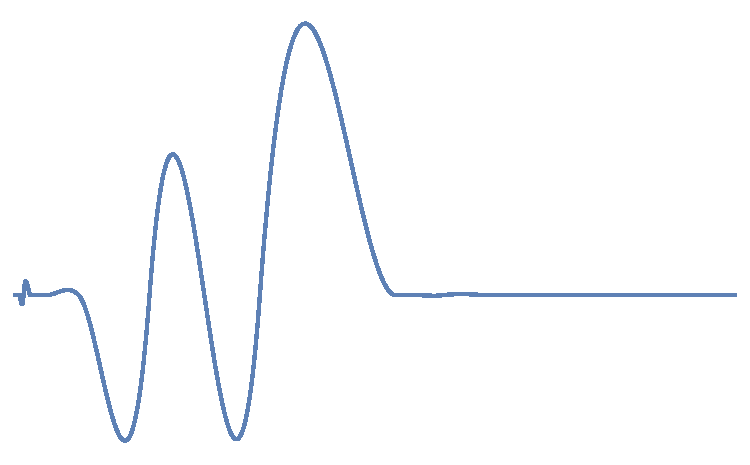
\includegraphics[width=.9\linewidth]{figures/int_oscillations.pdf}
		\end{figure}
 	\end{column}
 
 	\begin{column}{.5\linewidth}
% 		Connection between Num.Analysis and Experiment.
 	%	$$f_r - \text{laser relaxation frequency}$$
 		What about LF instead of HF?..
 		\begin{itemize}
 			\iitem{For semi-conductors laser $f_r \sim 1 \ \text{GHz}$;}
 			\iitem{For erbium-doped fiber ring laser (EDFRl) $f_r \sim 10 \text{kHz}$;}
 			\iitem{However, its hard to work with it.}
 		\end{itemize}
	\end{column}
	\end{columns}
